\chapter{随机网络生成器的设计及实现}
要运行Caffe,首先需要先创建一个模型(model),Caffe里自带了不少常用的神经网络模型,而一个模型由多个层(layer)构成,每一个层又包含多个参数,每一个层的参数都定义在caffe.proto这个文件内。因此,想要生成一个可以用于验证的模型,我们必须首先生成一个符合结构要求并含有参数定义的prototxt。
\section{随机网络生成器的设计}
\subsection{prototxt的概述}
prototxt是配置文件,是Caffe中用于描述网络参数以及网络结构的文件。这个文件里不包含对网络训练的权值,相当于一个网络构架。著名的AlexNet网络的prototxt的前四层以及其可视化如\autoref{fig:AlexNet}所示。因此,为了得到一个完整的随机网络,我们应该考虑先生成一个prototxt文件。

\begin{figure}[!htbp]
\centering 
\subfloat[AlexNet网络的prototxt]{
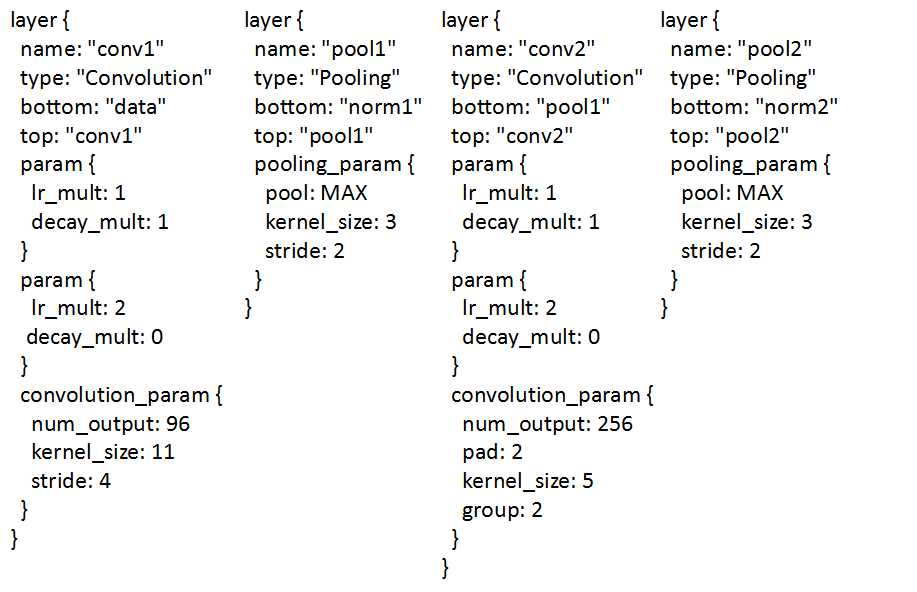
\includegraphics[width=12cm]{Alexnet2.jpg}}
\\
\subfloat[AlexNet网络的可视化]{
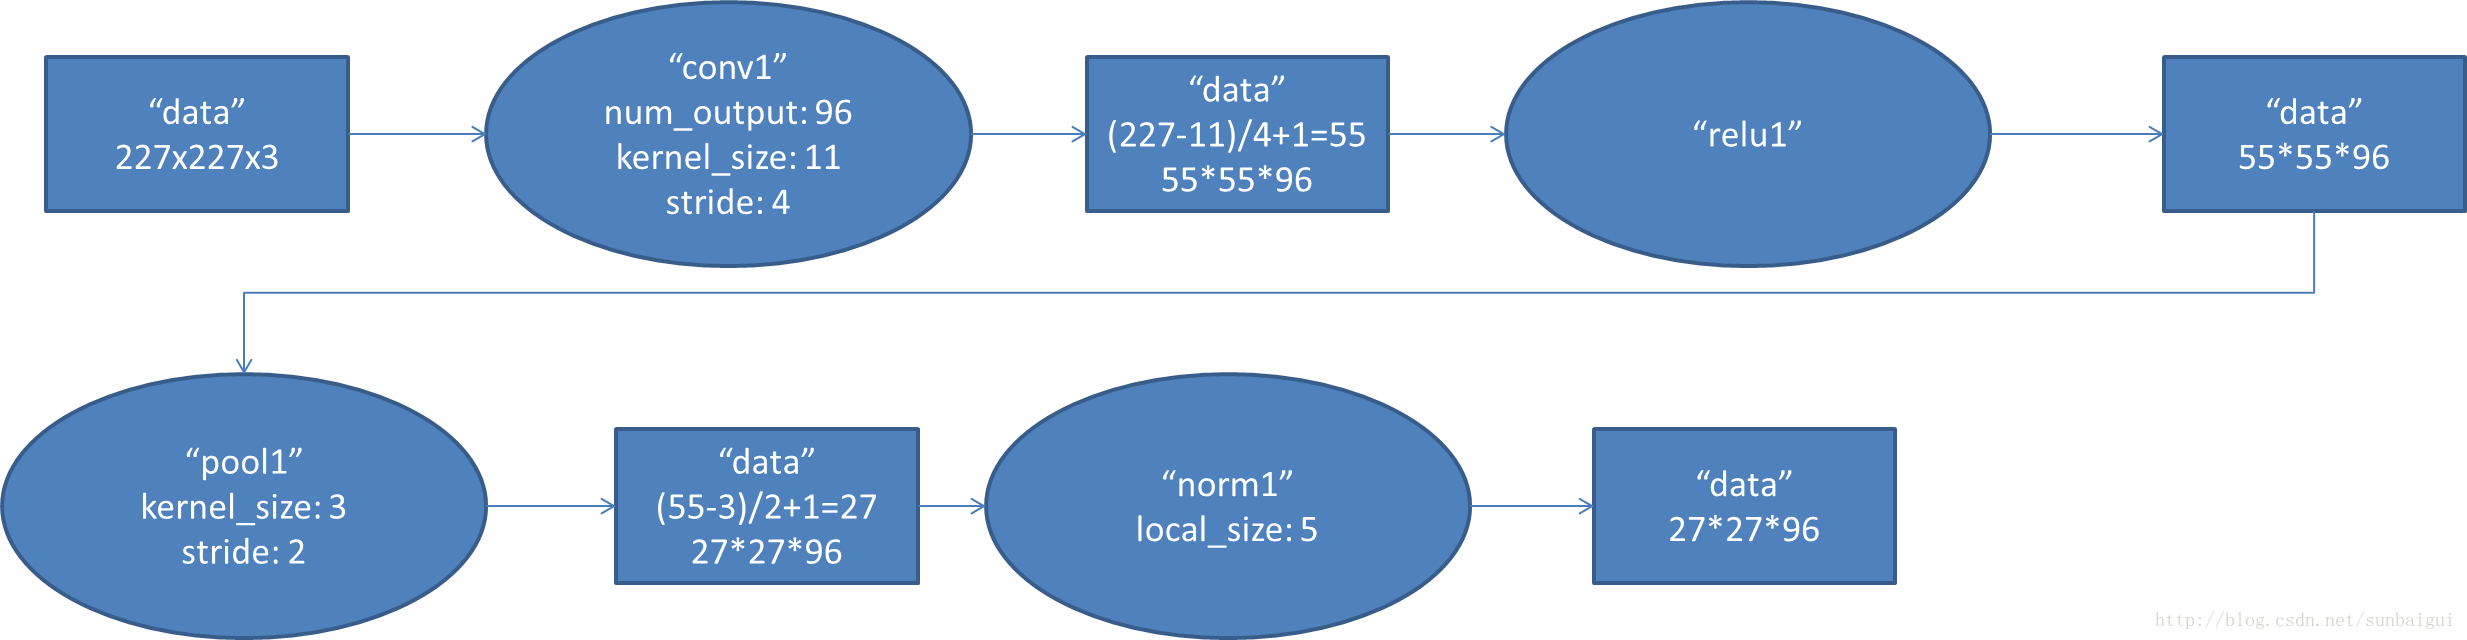
\includegraphics[width=12cm]{Alex1.png}}
\caption{AlexNet网络图}
\label{fig:AlexNet}
\end{figure}

\subsection{随机网络生成器的数据结构}
在我们神经网络生成器当中,有三个主要的数据结构,其一是用于描述网络中最基本粒子“层”的数据结构layer,另一个则是用于描述数据在层之间传递方法的数据结构blob\underline{ }shape。第三个则是用于读取,判断用户对网络结构需求的数据结构struct\underline{ }limit。

下面,我们分别介绍这三个数据结构。
首先,对于blob\underline{ }shape,这是一个一个密集的n维(n $\leq$ 4)阵列,在神经网络中,这代表神经元和偏置(bias)。

在Caffe中也拥有类似的数据结构Blob,用于封装了并在层与层之间传递运行时的信息,提供了CPU和GPU的同步。从数学上来说,Blob就是一个N维数组,是Caffe中的数据操作基本单位,就像matlab中以矩阵为基本操作对象一样。只是矩阵是二维的,而Blob是N维的。N可以是2,3,4等等。对于图片数据来说,Blob可以表示为(N$\times$C$\times$H$\times$W)这样一个4维数组。其中N表示图片的数量,C表示图片的通道数,H和W分别表示图片的高度和宽度。当然,除了图片数据,Blob也可以用于非图片数据。比如传统的多层感知机,就是比较简单的全连接网络,用2维的Blob,调用innerProduct层来计算即可。

而为了与Caffe提供的接口相对应,也为了保证生成网络连接方式的合理性,我们的blob\underline{ }shape也拥有和Caffe中Blob类的类似结构。在我们随机网络生成器中,网络内层与层之间的数据,是用blob\underline{ }shape来表示和运算。它的维度会根据网络参数与结构的类型不同而不同。例如,卷积操作取一个四维的blob\underline{ }shape进行输入,而输出一个四维的blob\underline{ }shape,而全连接操作则取一个四维blob\underline{ }shape进行输入,输出一个二维blob\underline{ }shape。

\begin{figure}[!htbp]
\centering
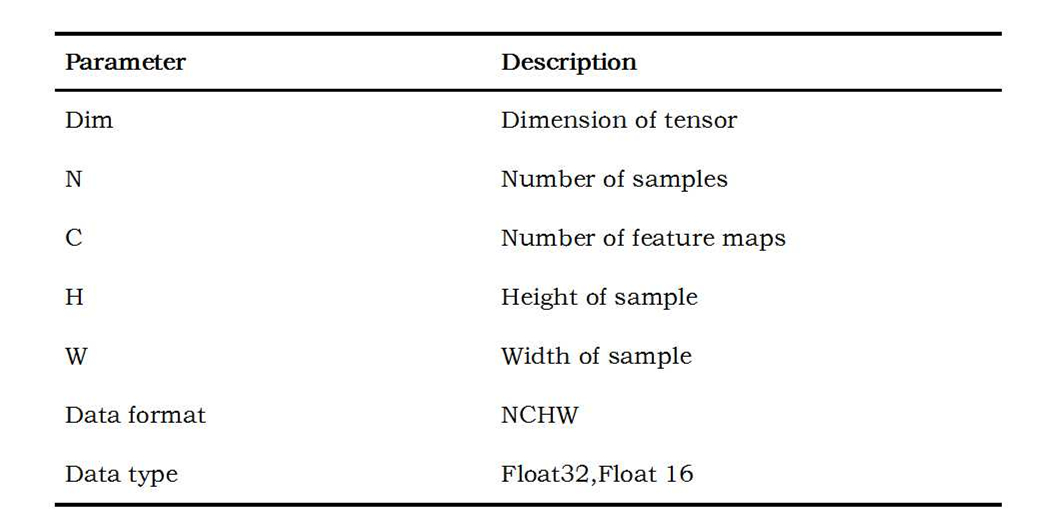
\includegraphics[width=12cm]{Tensor_Structure.jpg}
\caption{blob shape的参数}
\label{fig:Tensor_Structure}
\end{figure}

blob\underline{ }shape描述的属性和参数如\autoref{fig:Tensor_Structure}所示,\emph{N,C,H,W}表示四个维度的大小,其中\emph{N}表示样本数,\emph{C}表示特征映射的数量,也就是图片中通道数,而\emph{H,W}分别表示特征映射的高与宽,每一个数据的数据类型是一个枚举类型变量,用于表示张量的数据格式,这些字母的顺序代表了的blob\underline{ }shape数据排列。

值得注意的是,和Caffe中的Blob相比,我们的blob\underline{ }shape还有一个参数(Dim)用于描述blob\underline{ }shape的维度。对于维度小于4的blob\underline{ }shape,我们也可以用相同的格式来表示。例如,一个二维的blob\underline{ }shape,我们将其H与W设为1,而依靠Dim参数区分H与W都为1的四维blob\underline{ }shape,这样的好处是,我们可以保证数据的传递的有效性,同时也保证了所有的blob\underline{ }shape在网络的传递过程中计算形式上都具有相同的维度,而(Dim)这一参数可以让我们有效地分辨出该数据的实际数值,有效避免了误差。

\begin{figure}[!htbp]
\centering
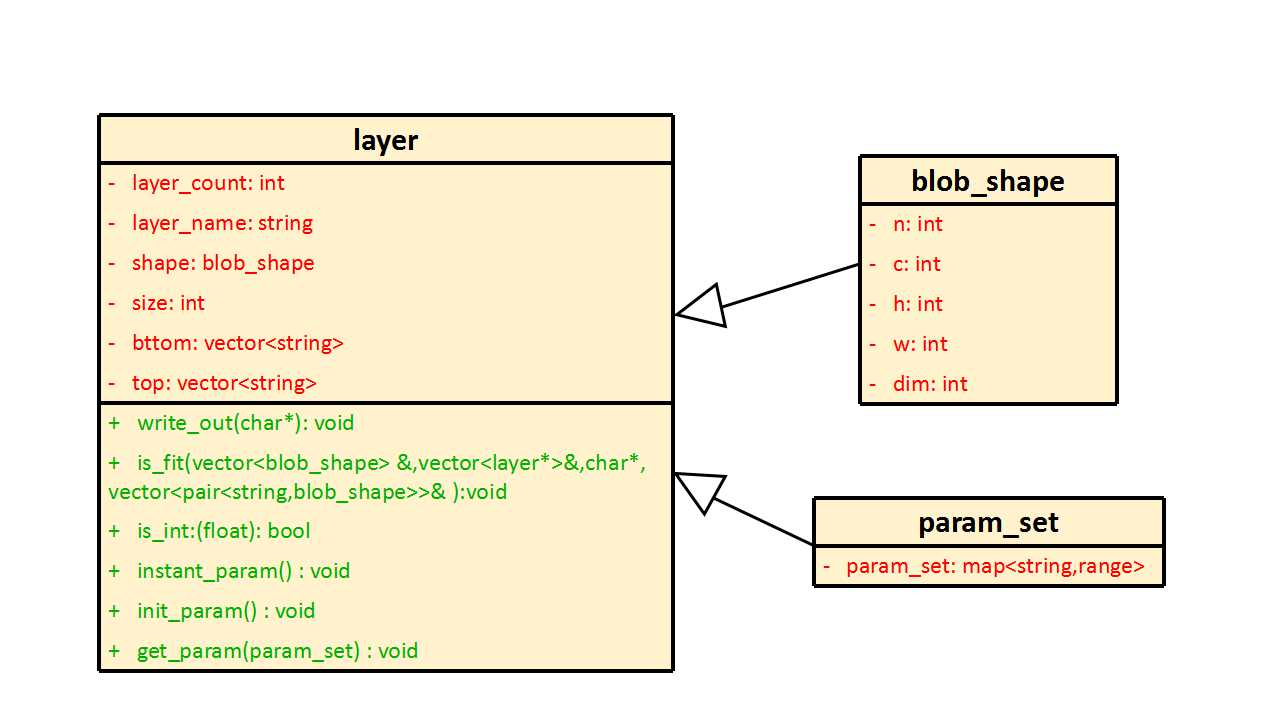
\includegraphics[width=12cm]{layer_blobshape.jpg}
\caption{layer与blobshape的类图}
\label{fig:layer_blobshape}
\end{figure}

对于另一个主要的数据结构——层(layer)来说,神经网络的层是一个独特的概念,这不但代表了一个操作,同时也包含了这个操作的参数,是网络模型的组成要素和基本单位。在Caffe中,proto.prototxt文件记录了每个层的参数种类,但Caffe中layer类用作层与层的运算与数据的传递,而非网络的生成。于是,在我们的随机网络生成器中,层(layer)被声明为一种新的类。这个类里面的变量与方法如\autoref{fig:layer_blobshape}所示。

其中write\underline{ }out方法用来打印网络结构,is\underline{ }fit方法则用于判断单个层(操作)所连接的位置。instant方法和get\underline{ }param方法用于初始化参数范围,前者的初始化是根据设计者估计的参数来设置的,而后者的初始化则是由用户设定的,后者的优先级高于前者,最后由instant方法在范围内随机得到参数,随机参数的类型(整数或者浮点数)由is\underline{ }int控制。

\begin{figure}[!htbp]
\centering
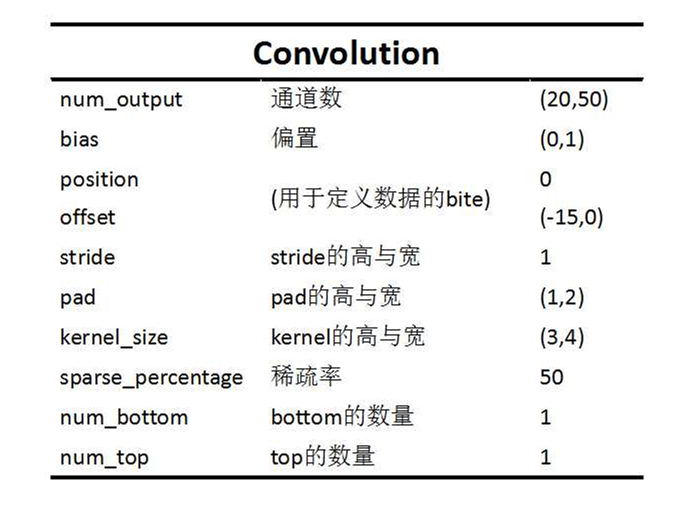
\includegraphics[width=12cm]{conv_param.jpg}
\caption{卷积层的参数类图}
\label{fig:conv_param}
\end{figure}
对神经网络来说,每一个操作(operator)都对应了大量的参数,网络中的layer与每一个operation一一对应。因此也会有众多的参数来描述层的特性。

我们以卷积层(conv\underline{ }layer)为例,说明卷积层内的参数。如\autoref{fig:conv_param}所示,卷积层内有10个参数(后期还可以根据用户的需求进行添加),其中num\underline{ }output,kernel\underline{ }size用于描述核的通道数与长和宽,而pad即stride则用于描述卷积操作中,核(kernel)的具体操作,sparse\underline{ }percentage用于定量描绘稀疏图的概率,这里的每一个参数都在神经网络的卷积操作中有意义,使得程序具有较强的可读性。

第三个数据结构struct\underline{ }limit是用于处理随机神经网络生成器中的结构要求,第一个作用是读取用户单层结构的概率分布,从而按照概率生成所需要的网络,第二个作用则是读取用户输入的串(即给定的layer序列、多层结构)以及串的生成概率,在判断串合法的情况下,生成具有特定连接方式的神经网络。struct\underline{ }limit类里面的变量与方法如\autoref{fig:struct_limit_lei}所示。

其中rule是用于读入用户定义规则的结构体,而snake类则定义了一系列规则,其中add方法用于添加新的规则,而dadj\underline{ }snake方法则用于调整连接规则(例如conv-mlp与mlp-pooling规则可以合成conv-mlp-pooling一条规则)而struct\underline{ }limit继承了两者,用于调配规则,其中series参数用于记录串的形式信息,而rule参数则用来记录用户所提供的生成规则,而check\underline{ }rule方法用于判断合法性。

\begin{figure}[!htbp]
\centering
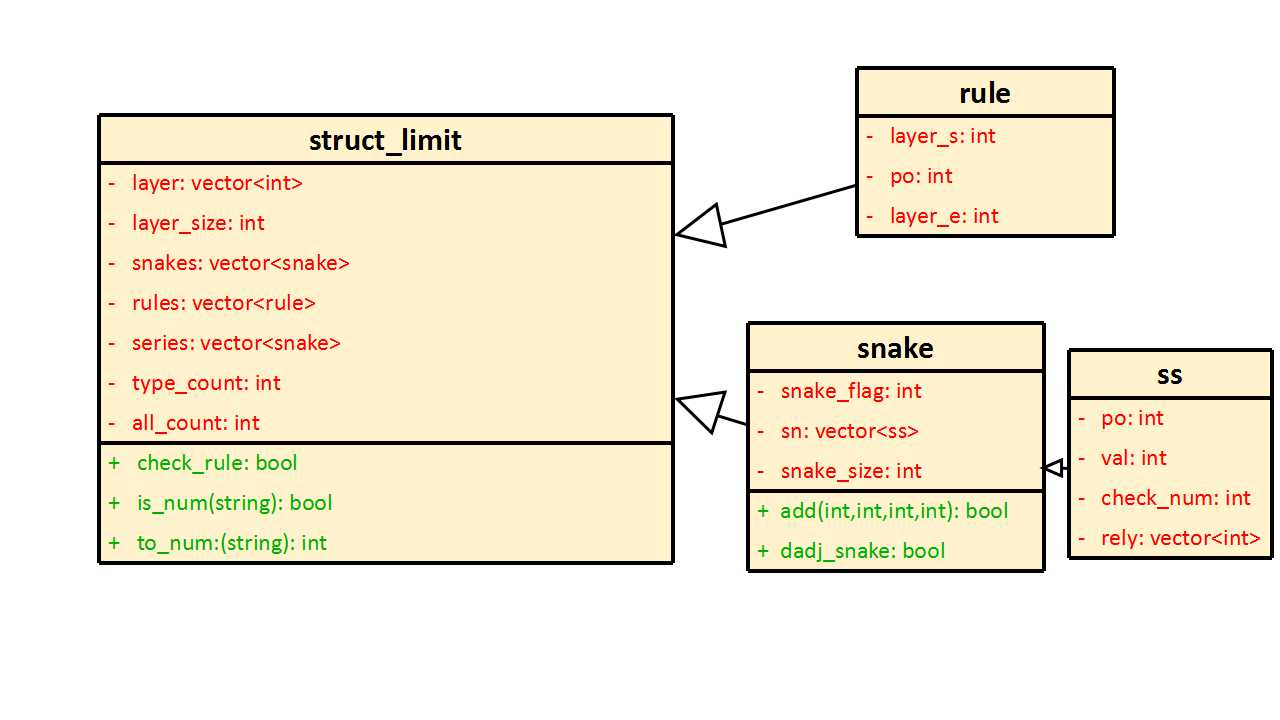
\includegraphics[width=12cm]{struct_limit_lei.jpg}
\caption{struct limit的类图}
\label{fig:struct_limit_lei}
\end{figure}

\subsection{网络的建立}
网络是由层(layer)构成,而blob\underline{ }shape封装了数据从layer一层一层输入再输出。而数据数据能否作为一个层的输入是取决于数据的维度、数值以及层的参数,而数据的输出则在层中根据层的种类与参数进行计算与调配。

卷积层是卷积神经网络(CNN)最重要的一种层的类型,它需要一个四维blob\underline{ }shape作为输出,并输出一个四维blob\underline{ }shape。张量的操作通过层来进行,卷积层的参数类型如\autoref{fig:conv_param}所示,一个blob\underline{ }shape传入卷积层后,N值保持不变,C值被卷基层的number\underline{ }output所取代,而H和W则由\autoref{eq:1.1}与\autoref{eq:1.2}计算:
\begin{equation}\label{eq:1.1}
H=\lceil \frac{H_{i}-K_h+1+2P_{h}}{S_{h}}\rceil
\end{equation}
\begin{equation}\label{eq:1.2}
W=\lceil \frac{W_{i}-K_w+1+2P_{w}}{S_{w}}\rceil
\end{equation}
其中$H_{i}$和$W_{i}$代表输入张量的H和W,$K_h$与$K_w$则代表了kernel的长和宽,而$P_h$,$P_w$则代表了pad的长和宽,这些都能在层的参数中得到,之后将得到的新的张量存储在shape中传向网络里更深的位置(层)内。

在blob\underline{ }shape的传入与输出过程中,is\underline{ }fit函数能控制输入的合法性,例如对于平常的卷积层,我们需要保证输入的blob\underline{ }shape是四维的,同时,输出的blob\underline{ }shape里,每一个成员变量都需要大于0,即还应该满足\autoref{eq:1.3}与\autoref{eq:1.4}:
\begin{equation}\label{eq:1.3}
\lceil H_{i}-K_h+1+2P_{h}\rceil >0
\end{equation}
\begin{equation}\label{eq:1.4}
\lceil W_{i}-K_w+1+2P_{w}\rceil >0
\end{equation}
对于一些操作复杂的层来说is\underline{ }fit函数还取到了生成补充层的作用,例如eltwise层需要输入多个blob\underline{ }shape,同时保证输入blob\underline{ }shape的四个维度都相等,而lstm\underline{ }unit层则既输入多个blob\underline{ }shape,同时也输出多个blob\underline{ }shape,进一步的,我们还可以根据库的要求、乃至硬件的要求调整is\underline{ }fit函数,使得该程序具有很好的可扩展性。
\section{随机网络生成器的实现}
\subsection{随机网络生成器的运行}
主函数首先读取struct\underline{ }limit以及param\underline{ }limit两个文件,前者用于描述网络的结构分布,即网络的深度以及每一类型的层在本次随机网络生成中所占有的比例,后者则用于描述不同层中参数的限制。这些结构分布与参数限制都根据用户的验证需求自行限制。另外,除了每次进行单个层的生成与连接外,还可以把多个层构成串一并连接并生成。例如,我们可以要求每一个卷积层(convolution)后面,连接的都是一个全连接层(mlp),这样子尽可能满足了用户的验证需求,也给程序的维护带来了便利。

\begin{figure}[!htbp]
\centering 
\subfloat[网络结构限制]{
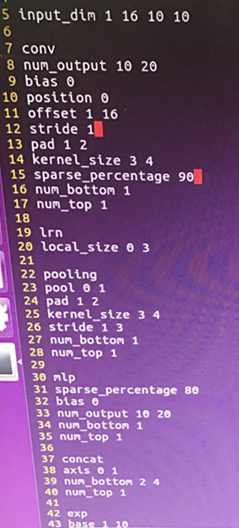
\includegraphics[width=4.5cm]{param_limit.jpg}}
\subfloat[网络参数限制]{
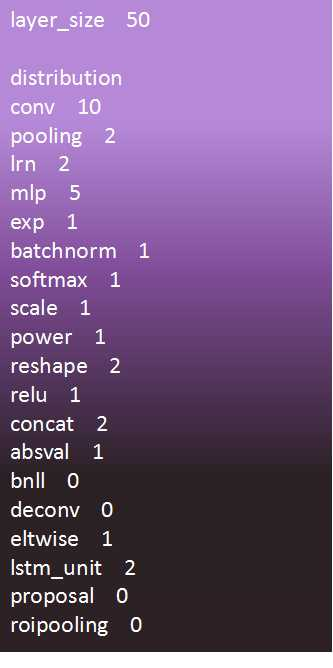
\includegraphics[width=4.5cm]{struct_limit.jpg}}
\caption{proto的运行}
\label{fig:limit}
\end{figure}
\section{caffe\underline{ }model的生成}

在读取参数后,主函数根据用户的需求按规则生成我们所需要的网络,并调用write\underline{ }out方法从而打印生成具有网络信息的prototxt文件。我们现在得到了网络信息,然而这个网络还是一个“空架子”,我们接下来先根据每一个层的连接方式,为网络补充上权值,我们写了一个create\underline{ }model函数,主要的作用就是调用Caffe提供的caffe\underline{ }param接口(caffe\underline{ }param是caffe提供的一个记录网络结构与权值并能直接生成caffe\underline{ }model的类),初始化一个Net类,在Net中我们将权值初始化,再赋值传回param类中,而后net\underline{ }param可以直接将网络结构以及权值写入caffe\underline{ }model中,至此,我们生成一个具有随机权值的真实网络,简单的说就是我们将一个“空架子”给“填充”了。这样子,便生成了我们所需要的 caffe\underline{ }model。

\subsection{生成已有的常用网络}
在前文中,我们已经介绍了随机网络模型的生成流程,虽然已有的常用网络(例如Lenet,Alex等)是随机网络模型的子集,但常用网络的训练效果已得到同行的验证,因此在我们神经网络处理器测试框架的测试中,具有一定的代表性,同时将已有的常用网络单独测试也可以增强开发者的信心。

对于常用网络,Caffe里面已经给出了现有的prototxt,甚至也有提供已经训练好的caffe\underline{ }model,因此,我们无需再去生成。(事实上,我们的随机网络模型生成器也可以按照给定的串生成常用网络),之后调用Caffe提供的caffe\underline{ }param接口,便可以生成具有随机权值的常用网络模型了。

\subsection{测试框架数据库的建立}
高效的测试需要有数据库来支持。对于神经网络处理器编译器的验证来说,由于bug主要出现在指令集中,由于神经网络处理器的特殊性,即使是同一条指令,不同的参数,指令的生存周期变化很大,且需要访问的存储范围变化也很大,所以我们的数据库里应该记载了完整的神经网络结构。我们的数据库应该由如下几个层次构成:

1.单个层随机参数的指令,因为随着库能支持的网络越来越多,需要验证的网络种类也会越来越复杂,因此,我们需要对网络的最基本构造——层进行单独测试。因此,对于每一种新的层,我们应该把单层的网络加入到库中。

2.已有的常用网络,常用的网络具有代表性,同时验证常用网络也会给予开发者信心,因此我们会收集其他同行使用过的网络,在库支持的前提下,对其进行验证。

3.之前出过错的网络结构。由于神经网络结构的复杂性,因此修正了一个错误有可能会导致其他错误,将这些corner case 收集,在每一次改良调试库之后,优先对这些网络结构进行测试,可以较容易的发现错误。这里也运用到了前文中介绍的回归测试的软件验证思想。
\section{本节总结}
第四章介绍了神经网络处理器编译器测试框架中最重要的随机网络生成器的实现。吸取了编程框架Caffe中数据结构的优点并对其结构进行改良,将层的连接方式以及网络的构建融入网络生成器的创建当中,并实现了一系列方法用于满足用户对结构以及参数的要求,最后,建立了一个数据库用于保证测试的高效性,同时阐述了数据库的设计思想。